\documentclass[12pt, a4paper]{report}
\usepackage[utf8]{vietnam}
\usepackage{array, makecell}
\usepackage{graphicx, graphics}
\renewcommand\theadfont{\bfseries}


\begin{document}
Hệ thống quản lý sinh viên khoa/viện trường đại học Bách khoa Hà Nội
% Yêu cầu chức năng (Function requiment): mô tả các chức năng mà phần mềm hệ thống cung cấp
% Yêu cầu phi chức năng (Non-Function requiment): mô tả các ràng buộc đặt lên dịch vụ và quá trình phát triển hệ thống (về chất lượng, về môi trường, chuẩn sử dụng, qui trình phát triển)
\chapter{Khảo sát hệ thống}
Mỗi năm trường đại học Bách khoa Hà Nội tuyển sinh khoảng gần 8000 sinh viên (số liệu năm 2022 ), với nhu cầu phục vụ các sinh viên một cách đầy đủ nhất\\
Công tác quản lý sinh viên (kết quả học tập) của sinh viên đóng vai trò hết sức quan trọng đối với hoạt động của một khoa trong các trường đại học.
% \section{Hệ thống cũ}

% \section{Yêu cầu hệ thống mới}
% Hệ thống có thể phục vụ lượng lớn khoảng 2000
% % (150*16) 
% sinh viên các khoa(viện) cùng lúc, có các chức năng như:
% \begin{itemize}
% 	\item Thể hiện được mô hình tổ chức sinh viên theo khoá, theo lớp, các ngành đào tạo
% 	\item Quản lý điểm (CPA) cập nhật qua các học kì
% 	\item Hệ thống có thể xuất ra các báo cáo thống kê tình trạng học tập sinh viên dựa trên số điểm (CPA), số tín chỉ nợ, đưa ra mức cảnh cáo
% 	\item Hệ thống có chức năng đăng ký form đồ án, thực tập
% 	\item Tìm kiếm vị trí thực tập về các mảng cụ thể, có thông tin liên hệ với giảng viên, doanh nghiệp.
% \end{itemize}
\section{Yêu cầu chung đối với phần mềm}
\subsection{Yêu cầu người sử dụng}
\begin{itemize}
  \item[-] \textit{Các chức năng của phần mềm:} phải tuân theo quy chế, quy trình đào tạo của trường đại học Bách khoa Hà Nội.
  \item[-] \textit{Phần mềm phải có giao diện thân thiện:} để mọi người đều có thể sử dụng được, không nhất thiết phải là người trong ngành công nghệ thông tin.
  \item[-] \textit{Hệ thống phải dễ sử dụng, quản lý:} đảm bảo tốt cho việc sử dụng phần mềm để quản lý cũng như tra cứu cùng thời điểm với số lượng lớn người sử dụng.
  \item[-] \textit{Hệ thống phải có khả năng bảo mật tốt:} tất cả mọi thông tin cá nhân chỉ có người được phân quyền mới được phép xem và chỉnh sửa.
  \item[-] \textit{Hệ thống phải có chức năng phục hồi, sao lưu dữ liệu thường xuyên:} tránh tình trạng mất, hỏng, sai lệch dữ liệu.
  \item[-] \textit{Hệ thống cần có khả năng mở rộng, nâng cấp trong tương lai:} để có thể thay đổi cho phù hợp với yêu cầu công tác quản lý.
  \item[-] \textit{Chi phí cho hệ thống (phần mềm, phần cứng, nhân sự vận hành) phải hợp lý:} không vượt quá ngân sách của trường nhưng vẫn đáp ứng được yêu cầu công việc. 
\end{itemize}
\subsection{Yêu cầu hệ thống}
\textbf{Yêu cầu chức năng}:
\begin{itemize}
  \item Chức năng quản lý hệ thống: cho phép người quản trị hệ thống có thể quản lý người sử dụng, phân quyền, quản lý danh mục và vận hành hệ thống.
  \item Chức năng quản lý thông tin: cho phép các bộ phận, phòng ban thực hiện cập nhật và quản lý thông tin của các sinh viên viện mình.
  \item Chức năng tra cứu thông tin: cho phép người truy cập hệ thống có thể xem các thông tin mà đã được người quản trị phân quyền cho mình.
\end{itemize}
\textbf{Yêu cầu phi chức năng:}
\begin{itemize}
  \item Giao diện thân thiện, dễ sử dụng.
  \item Truy xuất dữ liệu nhanh, lưu trữ dữ liệu tốt.
  \item Tìm kiếm nhanh, thuận tiện.
  \item Hệ thống bảo mật cao.
  \item Đáp ứng được các yêu cầu nghiệp vụ.
\end{itemize}
\textbf{Yêu cầu miền ứng dụng:}
\begin{itemize}
  \item Chạy được trên các hệ điều hành khác nhau.
  \item Hệ quản trị cơ sở dữ liệu tập trung(SQL server)
  \item Giao diện thiết kế theo một chuẩn nhất định.
\end{itemize}

\chapter{Đặc tả yêu cầu bài toán}
\section{Mô tả yêu cầu}
\subsection{Yêu cầu hệ thống quản lý sinh viên}
Xây dựng phần mềm quản lý thông tin sinh viên:
\begin{enumerate}
	\item Phầm mềm có yêu cầu đăng ký/đăng nhập hệ thống.
	\item Phầm mềm có thông tin lưu trữ của sinh viên: CPA, số tín chỉ đã qua, số tín chỉ nợ.
	\item Phần mềm có thể thống kê, đánh giá theo các mức cảnh báo sinh viên.
	\item Chức năng đăng ký hướng dẫn đồ án, thực tập.
	\item Chức năng tạo CV
	\item Chức năng tìm kiếm giảng viên, đề tài đồ án, vị trí thực tập.
\end{enumerate}

\subsection{Hệ thống quản lý sinh viên}
\begin{itemize}
	\item Chức năng đăng ký thành viên:
	      \begin{itemize}
		      \item Mỗi sinh viên đăng ký tài khoản mới với tài khoản microsoft mail trường cấp.
		      \item Đăng ký trực tiếp từ giao diện khởi động hệ thống.
		      \item Tài khoản đó sau khi đăng ký thành công có thể đăng nhập vào hệ thống.
		      \item Khi đăng ký thành công thì mặc định đó là tài khoản sinh viên.
	      \end{itemize}
	\item Chức năng đăng nhập/đăng xuất hệ thống có phân quyền người dùng:
	      \begin{itemize}
		      \item Tài khoản đăng nhập hệ thống với đúng tài khoản và mật khẩu mà hệ thống cung cấp.
		      \item Có thể đăng nhập bằng tài khoản google gmail hoặc tài khoản facebook trước đó đã được liên kết với tài khoản đăng ký.
		      \item Tài khoản đăng nhập nếu không còn nhu cầu sử dụng hệ thống hoặc cần đăng nhập tài khoản khác có thể tiến hành đăng xuất.
	      \end{itemize}
	\item Chức năng lưu trữ thông tin:
	      \begin{itemize}
		      \item Sinh viên có thể cập nhật, lưu trữ các thông tin học tập của cá nhân: CPA, số tín chỉ đã qua, số tín chỉ nợ, thuộc lớp nào.
		      \item Cán bộ giảng viên phụ trách có thể xem danh sách lớp và xác nhận sinh viên.
	      \end{itemize}
	\item Chức năng cập nhật thông tin:
	      \begin{itemize}
		      \item Hệ thống cho phép người dùng thay đổi thông tin cá nhân của mình.
		      \item Admin có thể cấp lại mật khẩu cho người dùng.
	      \end{itemize}
	\item Chức năng thống kê, đưa ra mức cảnh báo:
	      \begin{itemize}
		      \item Hệ thống có thể đưa ra biểu đồ thống kê số lượng các sinh viên đang ở các mức cảnh báo 1, 2, 3 và các sinh viên chậm chương trình.
		      \item Hệ thống có thể xuất dữ liệu ra file excel, pdf.
	      \end{itemize}
	\item Chức năng đăng ký hướng dẫn đồ án, thực tập:
	      \begin{itemize}
		      \item Hệ thống cung cấp form đăng ký hướng dẫn đồ án, form đăng ký thực tập.
		      \item Giáo vụ có thể kiểm tra các form đã submit về.
		      \item Trưởng bộ môn có thể truy cấp để xếp thứ tự ưu tiên các sinh viên.
	      \end{itemize}
	\item Chức năng tạo CV:
	      \begin{itemize}
		      \item Hệ thống cung cấp form để sinh viên điền các thông tin cá nhân của mình: giới thiệu bản thân, CPA, định hướng nghề nghiệp, kỹ năng hiện có,...
		      \item Hệ thống nhận form submit và trả về một file word bản CV mẫu, sinh viên có thể tải xuống để xem, chỉnh sửa.
	      \end{itemize}
	\item Chức năng tìm kiếm giảng viên, đề tài đồ án, vị trí thực tập:
	      \begin{itemize}
		      \item Hệ thống cho phép tìm kiếm từ khoá theo tên giảng viên, từ đó đưa ra các đề tài mà giảng viên hướng dẫn
		      \item Hệ thống cung cấp danh sách các vị trí thực tập.
	      \end{itemize}
\end{itemize}

\section{Các tác nhân của hệ thống}
\begin{tabular}{|c|c|l|}
	\hline
	\thead{STT} & \thead{Tác nhân} & \thead{Chức năng}                                                    \\
	\hline
	1           & Admin            & \makecell[l]{- Quản trị hệ thống.                                    \\ - Phân quyền người dùng. \\ - Cấp lại mật khẩu cho người dùng.}\\
	\hline
	2           & Giáo vụ          & \makecell[l]{- Quản lý danh sách sinh viên.                          \\ - Quản lý form trả về.} \\
	\hline
	3           & Giảng viên       & \makecell[l]{- Quản lý danh sách sinh viên lớp.}                     \\
	\hline
	4           & Sinh viên        & \makecell[l]{- Đăng nhập, cập nhật thông tin.                        \\ - Sử dụng hệ thống, thực hiện điền form.}\\
	\hline
	5           & Người dùng       & \makecell[l]{- Người dùng hệ thống với chức năng đăng ký tài khoản.} \\
	\hline
\end{tabular}

\chapter{Biểu đồ phân cấp chức năng}
\begin{center}
	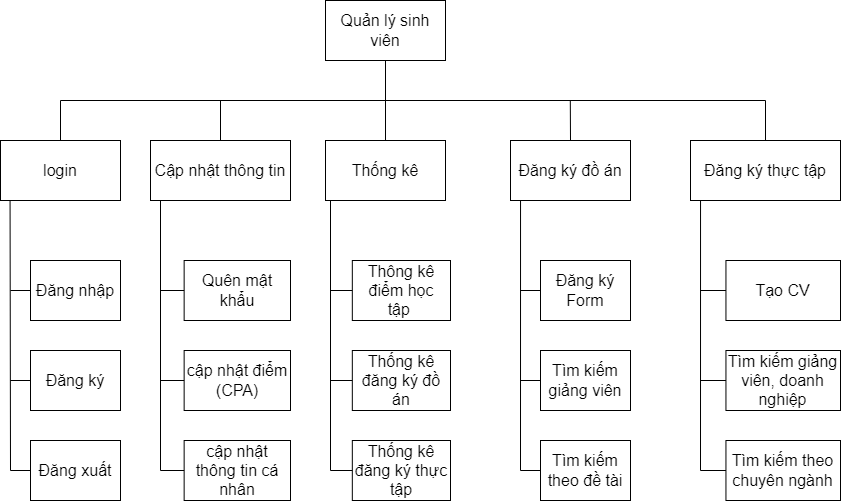
\includegraphics[width=1.1\textwidth]{image/BDPCCN.png}
	\begin{figure}
		\centering
		\caption{biểu đồ phân cấp chức năng}
	\end{figure}
\end{center}

\begin{center}
	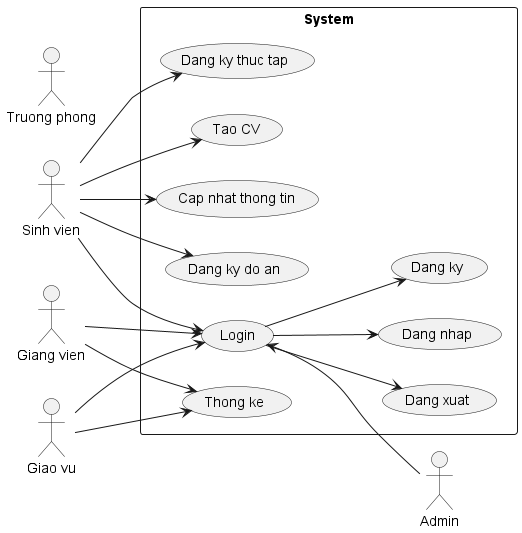
\includegraphics[width=.9\textwidth]{image/usecase.png}	
	\begin{figure}
		\centering
		\caption{biểu đồ usecase}
	\end{figure}
\end{center}

\end{document}
